
    \begin{figure}[]
        \centering
		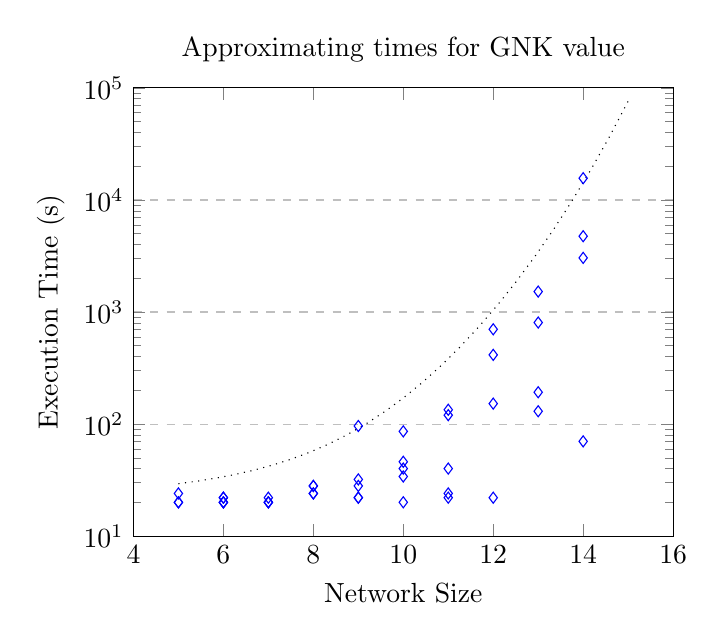
\begin{tikzpicture}
		\begin{axis}[
			title={Approximating times for GNK value},
			xlabel={Network Size},
			ylabel={Execution Time (s)},
			%xmin=0, xmax=0.25,
			ymin=10.00, ymax=100000.00,
			ymode=log,
			%xtick={0,0.05,0.1,0.15,0.2,0.25},
			%ytick={0,20,40,60,80,100},
			%yticklabel=$\pgfmathprintnumber{\tick}\%$,
			legend pos=south west,
			ymajorgrids=true,
			grid style=dashed,
			xticklabel style={/pgf/number format/fixed},
		]
		\addplot [domain=5:15,dotted] {20+exp(exp(x/6.2))};
		\addplot[color=blue,only marks,mark=diamond] coordinates {
(5,24.0643658638)
(5,20.0539109707)
(5,20.0425679684)
(6,22.0595200062)
(6,20.0396459103)
(6,22.0774619579)
(6,20.0592439175)
(6,20.0486550331)
(7,20.0611269474)
(7,20.0562839508)
(7,22.0582311153)
(7,20.0569791794)
(8,28.0723109245)
(8,28.0753469467)
(8,24.0676350594)
(8,24.0758149624)
(9,96.2227828503)
(9,22.0647089481)
(9,22.0649929047)
(9,28.080188036)
(9,32.0989830494)
(10,46.1140429974)
(10,40.1106638908)
(10,20.0607740879)
(10,34.0936999321)
(10,86.1996500492)
(11,22.0712139606)
(11,40.0975849628)
(11,120.281168938)
(11,24.0687379837)
(11,134.297913074)
(12,22.0656309128)
(12,414.870285988)
(12,152.341370821)
(12,701.464659929)
(13,1523.20846081)
(13,805.79351902)
(13,130.278774023)
(13,192.42149806)
(14,70.183686018)
(14,4745.82396007)
(14,3042.18855906)
(14,15641.2913539)
			}node[pos=0.8](endofplotsquare){} ;
		\end{axis}
		\end{tikzpicture}
		%\vspace{-18pt}
		\caption{Execution times in approximating the GNK value on random example networks of different sizes to 0.01 average magnitude of the error (relative the the magnitude of the estimated GNK value), between 8 independent estimations using \textsc{Join} method, with 20 seconds of validation time. Trend-line $20+\exp(\exp(n/6.2))$ indicates double exponential complexity}
		\label{fig:performance_graph2}
    \end{figure}



